
\documentclass[12pt,a4paper,titlepage,oneside]{article}
\usepackage[top=2.5cm, bottom=2cm, left=2.5cm, right=1cm]{geometry} 
% Font, accents
\usepackage[utf8]{inputenc}
\usepackage{fancyhdr}
\usepackage[T1]{fontenc}
\usepackage{float}    
% Interactive index
\usepackage{hyperref}
% Spanish titles
\usepackage[spanish]{babel}
% Attached files
\usepackage{attachfile}
\attachfilesetup{
  icon = Paperclip
}
% Fix curly verbatim apostrophes
\usepackage{upquote,textcomp}
% Make lists without bullets
\renewenvironment{itemize}{
 \begin{list}{}{
  \setlength{\leftmargin}{1.5em}
 }
}{
 \end{list}
}

%Customize things
\usepackage[margin=0pt,font=small,labelfont=bf]{caption}
\usepackage[pdftex]{graphicx}
\usepackage[usenames,dvipsnames]{xcolor}

% Sections and subsections colors
\usepackage{titlesec}
\titleformat{\section}
{\color{Blue}\normalfont\Large\bfseries}
{\color{Blue}\thesection}{1em}{}
\newcommand{\sectionbreak}{\clearpage}


% Document properties
\title{Facultad de Ingeniería\\Técnicas de Programación Concurrente I [75.59]}
\author{Federico Farina (90177) \\
Nicolás Vazquez (89172)}
\date{\today}
\hypersetup{
  colorlinks = true,
  urlcolor=blue,
  pdflang = es,
  pdfauthor = {Federico Farina},
  pdfproducer = {Federico Farina},
  pdfcreator = Texmaker,
  pdftitle = {TP2},
}

\begin{document}
   % code start
    \fancyhead[LE]{\leftmark} 
    \fancyhead[RO]{\rightmark} 
    \fancyhead[L]{Técnicas de Programación Concurrente I}
    \fancyhead[R]{TP2}    
    \renewcommand{\headrulewidth}{0.4pt} 
    \renewcommand{\footrulewidth}{0pt}
    % code end

    % set pagestyle to use fancy header and footer
    \pagestyle{fancy}


 \maketitle
  \setcounter{page}{1}
  \pagenumbering{roman}
  \tableofcontents

\newpage{}
\pagenumbering{arabic}
\setcounter{page}{1}

\section{Enunciado}

\subsection{Objetivo}

El objetivo de este proyecto consiste en implementar la simulación parcial del funcionamiento de una estación de servicio.

\subsection{Requerimientos Funcionales}

Esta simulacion abarcar a el funcionamiento de una estación de servicio. Los requerimientos funcionales son los siguientes:

\begin{enumerate}
\item 
La estacion de servicio cuenta con un número determinado de surtidores, un jefe de estación y un conjunto de empleados que atienden de a un auto por vez.
\item 
Tanto el número de surtidores disponibles como el número de empleados deben ser configurables y se establecen al inicio de la simulación.
\item
Cuando un auto llega a la estación de servicio es atendido en primer lugar por el jefe de estación quien asignará un empleado para atender al auto. Si no hay un empleado disponible, el auto se retira de la estación de servicio.
\item
La estación de servicio cuenta con dos tipos de clientes: regulares y VIP.
\item
El jefe de estación debe atender a los autos por orden de llegada de los mismos, salvo que llegue un cliente VIP, quien tendrá prioridad sobre los clientes regulares.
\item
Cuando el empleado recibe un auto de parte del jefe de estación, debe localizar un surtidor libre para atender al auto en cuestión. Si no encuentra ningú surtidor libre, deberá esperar hasta tanto se libere alguno.
\item
Una vez que el empleado obtiene un surtidor atiende al auto en cuestión. Mientras el empleado está atendiendo al auto no se puede utilizar el mismo surtidor para otro auto, ni el empleado es capaz de atender más de un auto a la vez.
\item
Finalmente, antes de que el auto se retire el empleado deberá cobrar el cargo correspondiente, el cual será almacenado en la caja de la estación de servicio.
\item
Todos los empleados guardan la recaudación en la misma caja y sólo un empleado puede utilizar la caja a la vez.
\item
Durante cualquier momento de la simulación, el administrador de la estación de servicio podrá consultar la recaudación guardada en la caja. Mientras lo hace, si algún empleado tiene recaudación para guardar, deberá esperar hasta que el administrador finalice su consulta.
\item
El administrador deberá tener prioridad sobre los empleados al momento de utilizar la caja.
\item
Se deberá poder trackear en el log de la simulación qué empleado atendió a qué auto y qué surtidor utilizó al hacerlo.

\end{enumerate}

 
\subsection{Requerimientos no Funcionales}

Los siguientes son los requerimientos no funcionales de la aplicación:

\begin{enumerate}
 \item
  El proyecto deberá ser desarrollado en lenguaje C o C++, siendo este último el  lenguaje de preferencia.
  \item
  La simulación puede no tener interfaz gráfica y ejecutarse en una o varias consolas de línea decomandos.
  \item
  El proyecto deberá funcionar en ambiente Unix / Linux.
  \item
La aplicación deberá funcionar en una única computadora.  
\item
El programa deberá poder ejecutarse en "modo debug", lo cual dejará registro de la actividad que realiza en un único archivo de texto para su revisión posterior.
\end{enumerate} 


Las facilidades de IPC que se podrán utilizar para la realización de este proyecto son las que abarcan la primera y la segunda parte de la materia.

\subsection{Tareas a Realizar}

A continuación se listan las tareas a realizar para completar el desarrollo del proyecto:

\begin{enumerate}
\item
 Dividir el proyecto en procesos. El objetivo es lograr que la simulación esté conformada por un conjunto de procesos que sean lo más sencillos posible.
\item
Una vez obtenida la división en procesos, establecer un esquema de comunicación entre ellos teniendo en cuenta los requerimientos de la aplicación. ¿Qué procesos se comunican entre sí?, ¿Qué datos necesitan compartir para poder trabajar?
\item
Tratar de mapear la comunicación entre los procesos a los problemas conocidos de concurrencia.
\item 
Determinar los mecanismos de concurrencia a utilizar para cada una de las comunicaciones entre procesos que fueron detectadas en el ítem 2. No se requiere la utilización de algún mecanismo específico, la elección en cada caso queda a cargo del grupo y debe estar debidamente justificada.
\item
 Realizar la codificación de la aplicación. El código fuente debe estar documentado.
\end{enumerate}
 
\subsection{Entrega} 

La entrega del proyecto comprende lo siguiente:

\begin{enumerate}
\item
Informe, se deberá presentar impreso en una carpeta o folio y en forma digital (PDF) a través del campus
\item
El código fuente de la aplicación, que se entregará únicamente mediante el campus
\end{enumerate}

La entrega en el campus estará habilitada hasta las 19 hs de la fecha indicada oportunamente.

El informe a entregar debe contener los siguientes ítems:

\begin{enumerate}
\item
Breve análisis del problema, incluyendo una especificación de los casos de uso de la aplicación.
\item
Detalle de resolución de la lista de tareas anterior.
\item
Diagrama que refleje los procesos, el flujo de comunicación entre ellos y los datos que intercambian.
\item
Diagramas de clases realizados.
\item
Diagrama de transición de estados de un empleado de la estación.
\end{enumerate}

\section{Objetivo}
El objetivo de este proyecto es el desarrollo de una aplicación conocida como ConcuStation.
Esta aplicación permitirá simular el funcionamiento de una estación de servicio. Al iniciar la aplicación, el usuario podrá decidir el número de empleados y surtidores que desee.
Los empleados atienden un auto por vez y almacenan la recaudación en una caja común. En todo momento se podrá consultar el saldo disponible en la caja.

\section{Análisis del problema}
Para el análisis del problema, se identificaron los actores que intervienen en el sistema. A continuación se presenta una breve descripción de cada uno.

\subsection{Actores}
\begin{enumerate}
\item[•] Jefe de estación: Encargado de recibir los autos que ingresan en la estación de servicio y asignar un empleado para su atención.
\item[•] Empleado: Encargado de atender los autos y almacenar la recaudación en la caja.
\item[•] Administrador: Consulta la recaudación disponible en la caja.
\end{enumerate}

\subsection{Casos de uso}
Se identificaron los siguientes casos de uso:

\begin{enumerate}
\item[•] Recibir auto: El jefe de estación recibe un nuevo auto que ingresa a la estación de servicio.
\item[•] Asignar empleado: El jefe de estación asigna un empleado disponible para atender el auto que ha ingresado a la estación de servicio.
\item[•] Atender auto: El empleado atiende un auto asignado previamente por el jefe de estación.
\item[•] Almacenar recaudación: El empleado almacena la recaudación obtenida al atender un auto en la caja de la estación de servicio.
\item[•] Consultar recaudación: El administrador de la estación de servicio consulta la recaudación contenida en la caja.
\end{enumerate}

\subsection{Caso de uso: Recibir auto}

\begin{enumerate}
\item \textbf{Descripción:} El jefe de estación recibe un nuevo auto que ingresa a la estación de servicio.
\item \textbf{Actores participantes}: Jefe de Estación
\item \textbf{Pre-condiciones}: -
\item \textbf{Flujo principal}
\begin{enumerate}
\item El auto ingresa a la estación de servicio
\item El auto se coloca detrás del último auto en ingresar a la estación de servicio
\item El auto espera a que el jefe de estación se encuentre libre
\item El auto es recibido por el jefe de estación
\item Fin del caso de uso
\end{enumerate}
\textbf{Post-condiciones:} El jefe de estación se encuentra libre
\end{enumerate}

\subsection{Caso de uso: Asignar empleado}

\begin{enumerate}
\item \textbf{Descripción:} El jefe de estación asigna un empleado para atender un nuevo auto. 
\item \textbf{Actores participantes}: Jefe de Estación, Empleado
\item \textbf{Pre-condiciones}: El auto debe haber sido previamente recibido por el jefe de estación.
\item \textbf{Flujo principal}
\begin{enumerate}
\item El jefe de estación busca un empleado libre para atender el auto
\item El jefe de estación asigna el auto al primer empleado libre que encuentre
\item Fin del caso de uso
\end{enumerate}
\item \textbf{Flujos de excepción}
\begin{enumerate}
\item No hay empleados disponibles para atender el auto
\begin{enumerate}
\item El auto se retira de la estación de servicio.
\end{enumerate}
\end{enumerate}
\textbf{Post-condiciones:} El auto ha sido asignado a un empleado o bien se ha retirado de la estación de servicio por no haber empleados disponibles. El empleado se encuentra ocupado atendiendo el auto y el jefe de estación se encuentra libre para recibir un nuevo auto
\end{enumerate}

\subsection{Caso de uso: Atender auto}

\begin{enumerate}
\item \textbf{Descripción:} El empleado atiende el auto asignado por el jefe de estación.
\item \textbf{Actores participantes}: Empleado
\item \textbf{Pre-condiciones}: El auto a atender debe ser previamente asignado por el jefe de estación. El empleado no puede estar ocupado atendiendo otro auto.
\item \textbf{Flujo principal}
\begin{enumerate}
\item El empleado busca un surtidor libre para atender el auto
\item El empleado determina el tiempo de carga según la capacidad del tanque de nafta del auto
\item El empleado carga nafta en el auto
\item El empleado libera el surtidor utilizado
\item Fin del caso de uso
\end{enumerate}
\textbf{Post-condiciones:} El surtidor utilizado por el empleado se encuentra libre
\end{enumerate}

\subsection{Caso de uso: Almacenar recaudación}

\begin{enumerate}
\item \textbf{Descripción:} El empleado almacena la recaudación resultante de la atención de un auto en la caja de la estación de servicio.
\item \textbf{Actores participantes}: Empleado
\item \textbf{Pre-condiciones}: El empleado debe haber terminado de cargar nafta en el auto.
\item \textbf{Flujo principal}
\begin{enumerate}
\item El empleado solicita el uso de la caja de la estación de servicio
\item El empleado espera hasta que se libere la caja de la estación de servicio
\item El empleado almacena la recaudación resultante en la caja de la estación de servicio
\item Fin del caso de uso
\end{enumerate}
\textbf{Post-condiciones:} La recaudación es almacenada en la caja y el empleado se encuentra disponible para atender un nuevo auto.
\end{enumerate}

\subsection{Caso de uso: Consultar recaudación}

\begin{enumerate}
\item \textbf{Descripción:} El administrador consulta la recaudación disponible en la caja de la estación de servicio.
\item \textbf{Actores participantes}: Administrador
\item \textbf{Pre-condiciones}: -
\item \textbf{Flujo principal}
\begin{enumerate}
\item El administrador solicita el uso de la caja de la estación de servicio
\item El administrador espera hasta que se libere la caja de la estación de servicio
\item El administrador consulta el saldo disponible en la caja de la estación de servicio
\item Fin del caso de uso
\end{enumerate}
\textbf{Post-condiciones:} El administrador conoce el saldo disponible en la caja de la estación de servicio.
\end{enumerate}

\section{Tareas realizadas}

\begin{enumerate}
\item Dividir el programa en procesos. El objetivo es lograr que cada programa participante este conformado por un conjunto de procesos que sean lo más sencillos posible.

\begin{itemize}
\item[•] Se crean dos procesos principales: Un proceso asociado a la vista (interfaz gráfica de usuario) y un proceso que controla el flujo de ejecución de la simulación.
\item[•] Se crea un proceso cada vez que entra un auto a la estación de servicio: Al ingresar es recibido por el jefe de estación, el cual busca algún empleado que se encuentre disponible para ser asignado a atender el auto. Si hay algún empleado disponible, se crea un nuevo proceso para atender el auto. La duración de la atención está determinada por la capacidad en litros del tanque de nafta del auto.
\end{itemize}

NOTA: En el caso de no haber empleados disponibles al ingresar un nuevo auto, no es posible atenderlo y el mismo se retira de la estación de servicio.

\item Una vez obtenida la división en procesos, establecer un esquema de comunicación entre ellos teniendo en cuenta los requerimientos de la aplicación. ¿Qué procesos se comunican entre sí? ¿Qué datos necesitan compartir para poder trabajar?

\begin{itemize}
\item[•] La vista se debe comunicar con el proceso principal para indicarle la capacidad y el tipo de auto que ha ingresado a la estación de servicio.
\item[•] El proceso principal y los procesos responsables de atender los autos que ingresan en la estación de servicio dejan el registro de su actividad en un único archivo de texto si el programa es ejecutado en modo debug. Este archivo debe ser compartido por todos los procesos.
\item[•] Cada vez que se lanza un proceso para atender un nuevo auto, el proceso escribe la recaudación resultante en una caja común. Esta caja es compartida por todos los procesos y por el administrador de la estación de servicio, el cual en todo momento puede consultar la recaudación contenida en la caja.
\item[•] La vista debe comunicar al proceso principal la finalización del tiempo de simulación. Este tiempo es controlado por la vista mediante un timer.
\end{itemize}

\item Tratar de mapear la comunicación entre los procesos a los problemas conocidos de concurrencia.

\textbf{Llegada de un nuevo auto y Jefe de Estación}

Este problema puede tratarse como un problema de Productor-Consumidor. El producto es la llegada de un nuevo auto, que se toma como un proceso aleatorio; y el consumidor es el jefe de estación, que ejecuta una lectura destructiva. La comunicación entre las dos partes está basada en una cola de mensajes que se escribe de manera asincrónica y se lee de manera sincrónica. De esta manera, el productor (proceso aleatorio) agrega al final de la cola de mensajes cada nuevo auto producido y el consumidor (jefe de estación) lo consume.

\textbf{Jefe de Estación-Empleados}

La relación entre los empleados y el jefe de estación puede verse como el problema de productores y consumidores. En este caso, los empleados son los que producen su disponibilidad y el jefe de estación la consume. 
La comunicación es asincrónica porque apenas se encuentre disponible un empleado, el jefe de estación lo utiliza para atender un nuevo auto.

\textbf{Administrador-Empleados con la caja}

Este problema puede verse como un problema de Lectores-Escritores. El recurso por el cual competir en este caso es la caja, en la cual el administrador lee y el empleado escribe. La prioridad es siempre para el administrador (Lector), lo que hace que cualquier empleado que esté esperando para escribir en la caja, tenga que esperar a que el administrador ejecute todas sus lecturas pendientes.
 
\item Determinar los mecanismos de concurrencia a utilizar para cada una de las comunicaciones entre procesos que fueron detectadas en el ítem 2. No se requiere la utilización de algún mecanismo específico, la elección en cada caso queda a cargo del grupo y debe estar debidamente justificada.

\begin{itemize}
\item[•] Si el programa es ejecutado en modo debug, se utiliza un Lock File para sincronizar correctamente la escritura de los procesos en el archivo de texto.
\item[•] El proceso principal se comunica con la vista por medio de una cola de mensajes. Al ingresar un nuevo auto, se puede determinar su capacidad mediante la interfaz gráfica de usuario. La vista escribe en la cola de mensajes dicha capacidad y el tipo de auto que ha ingresado a la estación de servicio y el proceso principal la lee para determinar el tipo de auto y el tiempo que necesita en ser atendido.
\item[•] Para determinar que surtidor se encuentra libre, se utiliza una memoria compartida cuyo tamaño coincide con la cantidad de surtidores que existan en la estación de servicio. Esta memoria es compartida por todos los procesos que se crean al asignar un empleado a atender un nuevo auto. Se utiliza un semáforo de exclusión mutua para sincronizar correctamente el acceso a este recurso.
\item[•] La caja es una memoria compartida por todos los procesos que se lanzan cada vez que ingresa un nuevo auto. Dado que estos procesos pueden ejecutarse concurrentemente, se utiliza un semáforo de exclusión mutua para la sincronización de la lectura y escritura en la memoria compartida.
\item[•] Para solicitar el uso de la caja, los empleados escriben un mensaje en una cola de mensajes que va almacenando las peticiones realizadas tanto por los empleados como por el administrador. Esta cola de mensajes es leída sincrónicamente por el encargado de administrar la caja; el cual asigna su uso a un empleado dependiendo de que existan peticiones o no del administrador. En caso de existir peticiones del administrador, los empleados deberán esperar hasta que el administrador haya terminado de consultar el saldo disponible en la caja.
\end{itemize}
\end{enumerate}

\section{Diagrama de casos de uso}
\begin{figure}[hbtp]
\begin{center}
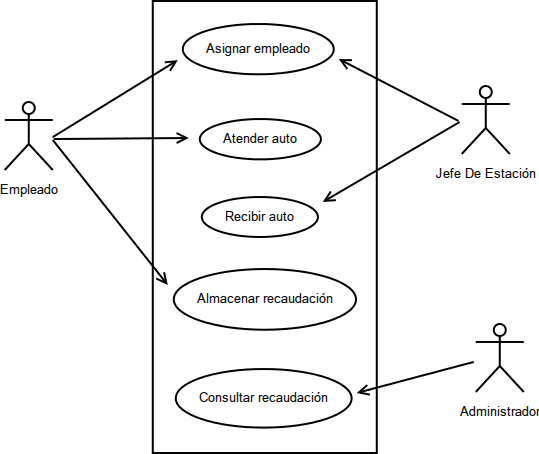
\includegraphics[scale=0.6]{diagramaDeCasosDeUso.png} 
\end{center}
\caption{Diagrama de casos de uso}
\end{figure}

\section{Diagrama de clases}
\begin{figure}[hbtp]
\centering
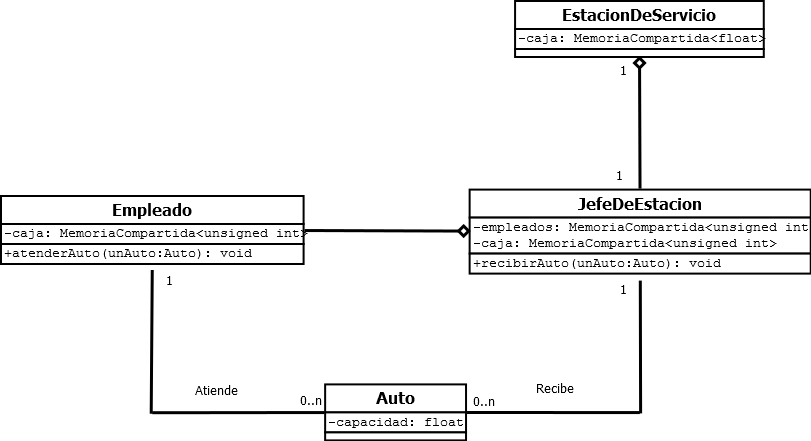
\includegraphics[scale=0.4]{diagramaDeClases.png}
\caption{Diagrama de clases}
\end{figure}

\section{Diagrama de estado}
\begin{figure}[hbtp]
\begin{center}
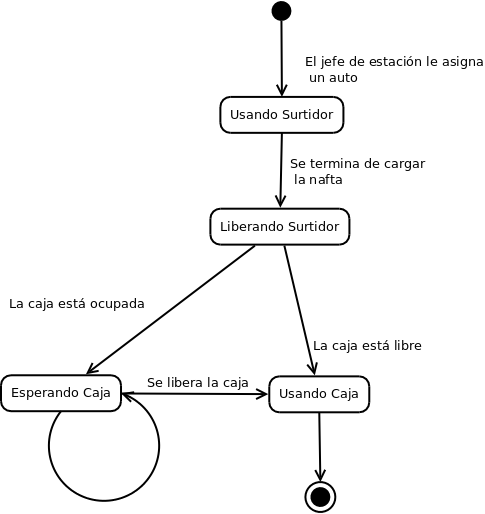
\includegraphics[scale=0.5]{diagrama_estado_empleado.png}
\end{center}
\caption[Long caption]{Diagrama de estado de un empleado}
\end{figure}

\section{Diagrama de procesos}
\begin{figure}[hbtp]
\begin{center}
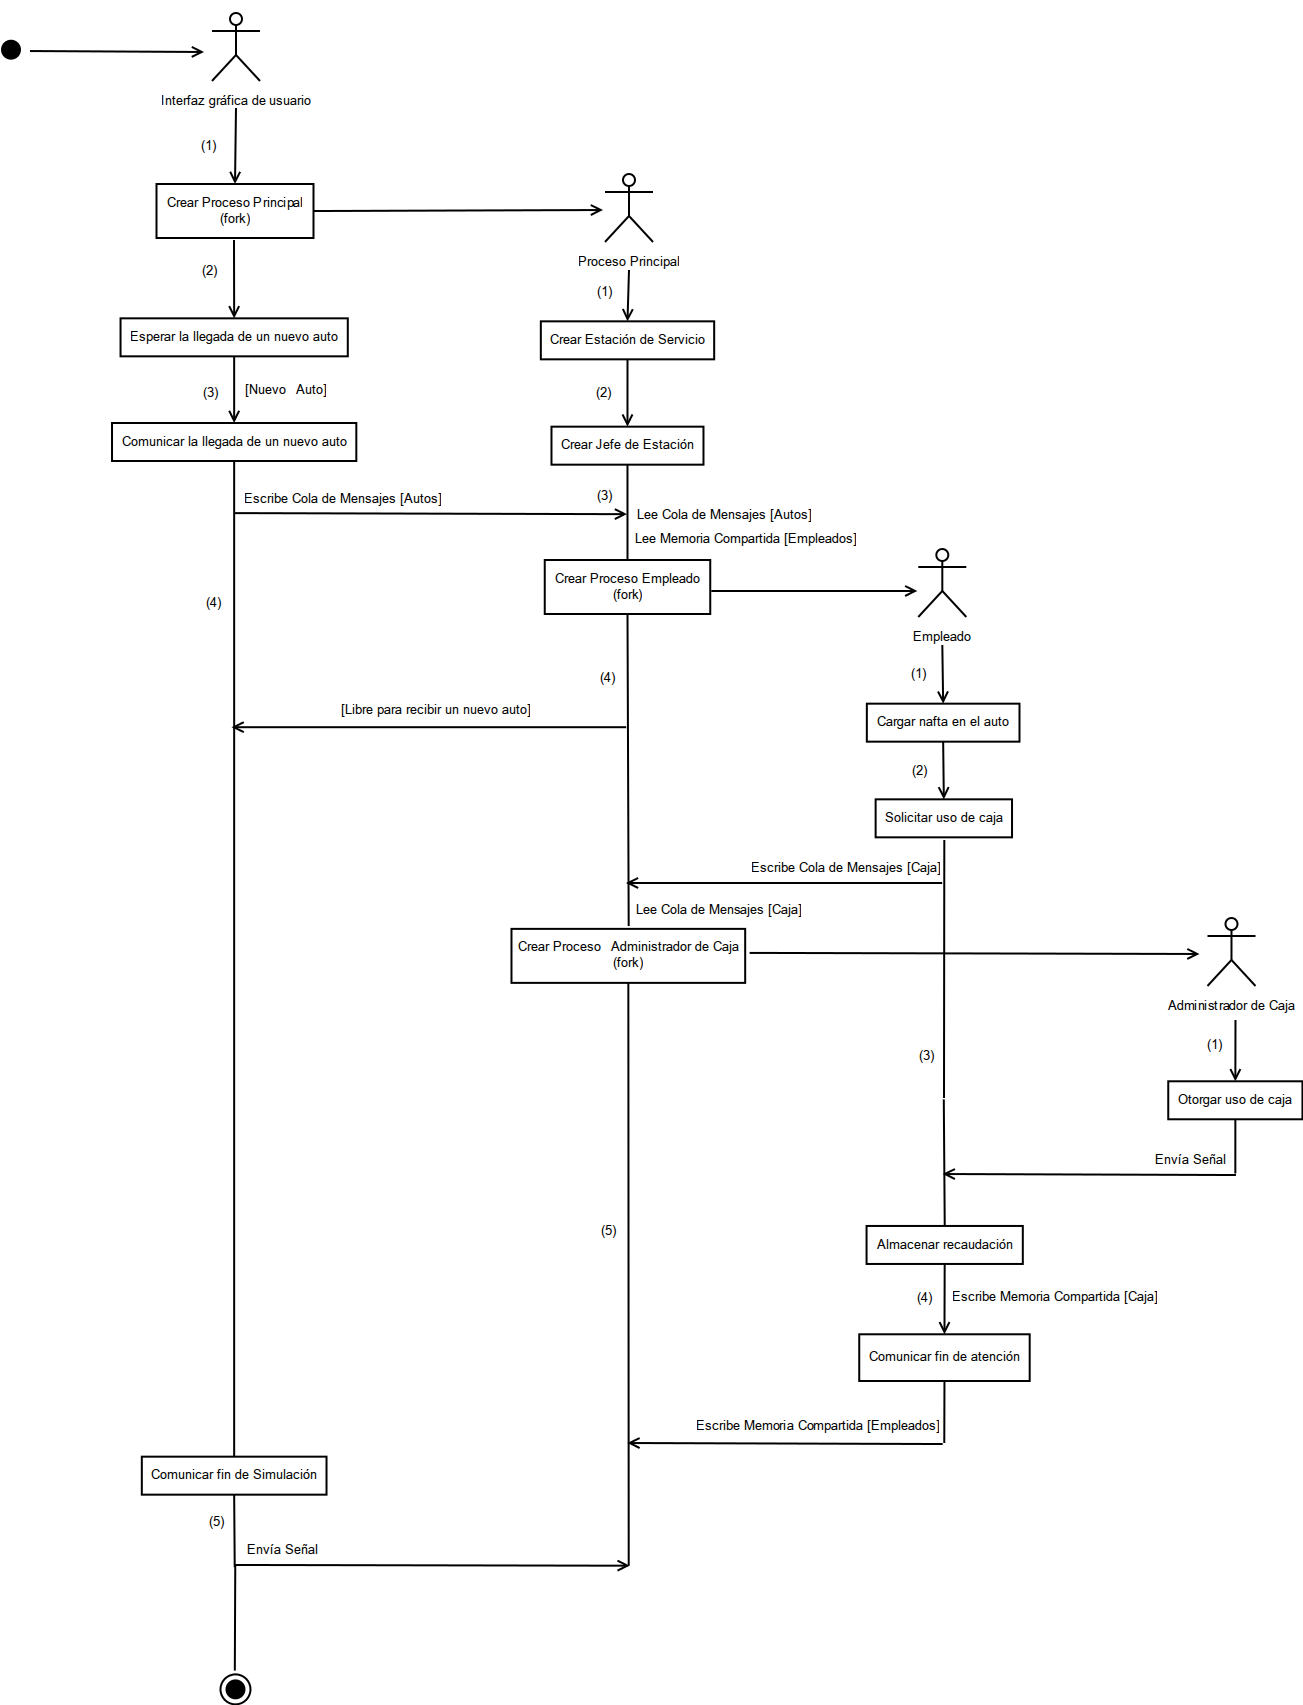
\includegraphics[scale=0.3]{diagramaDeProcesos.png} 
\end{center}
\caption{Diagrama de procesos}
\end{figure}

\end{document}